\documentclass[9pt]{IEEEtran}

\usepackage[english]{babel}
\usepackage{graphicx}
\usepackage{epstopdf}
\usepackage{fancyhdr}
\usepackage{amsmath}
\usepackage{amsthm}
\usepackage{amssymb}
\usepackage{url}
\usepackage{array}
\usepackage{textcomp}
\usepackage{listings}
\usepackage{hyperref}
\usepackage{xcolor}
\usepackage{colortbl}
\usepackage{float}
\usepackage{gensymb}
\usepackage{longtable}
\usepackage{supertabular}
\usepackage{multicol}
\usepackage[utf8x]{inputenc}
\usepackage{csquotes}
\usepackage[backend=biber, style=numeric]{biblatex}
\addbibresource{bibliography.bib}
\usepackage[T1]{fontenc}
\usepackage{lmodern}
\input{glyphtounicode}
\pdfgentounicode=1
\graphicspath{{./figures/}}
\DeclareGraphicsExtensions{.pdf,.png,.jpg,.eps}

% correct bad hyphenation here
\hyphenation{op-tical net-works semi-conduc-tor trig-gs}

% ============================================================================================

\title{\vspace{0ex}
Modeling Social Distancing with Reinforcement Learning}

\author{Nejc Ločičnik, Igor Nikolaj Sok, Leon Todorov, Andraž Zrimšek \vspace{-4.0ex}}

% ============================================================================================
\addbibresource{literature.bib}
\begin{document}

\maketitle

\section{Introduction}

The spread of infectious diseases is a significant challenge in both human and animal populations, prompting natural and artificial systems alike to develop mechanisms for minimizing transmission. Social distancing has emerged as a common adaptive behavior in nature, where organisms avoid close contact with infected individuals to protect themselves and their groups. This phenomenon has been observed across a variety of species and environments, suggesting it provides an evolutionary advantage in mitigating disease transmission risks. In response to the COVID-19 pandemic, social distancing also became a key public health strategy for humans, sparking interest in understanding how such behaviors might emerge and evolve autonomously in artificial agents.

Modeling disease transmission and social distancing behaviors in simulated environments can provide insights into the underlying dynamics of these processes, as well as offer potential applications in fields such as epidemiology, robotics, and swarm intelligence. Traditional approaches often rely on predefined rules to drive agent behaviors, limiting the complexity and adaptability of emergent patterns. By contrast, reinforcement learning (RL) provides a flexible framework where agents learn to navigate environments based on reward structures, allowing for more organic, adaptive behaviors that evolve in response to environmental pressures.

In this study, we aim to model social distancing behaviors using a reinforcement learning approach inspired by natural systems. Agents will learn to minimize disease transmission within a two-dimensional environment by adapting their interactions based on health information they exchange with one another. We will build on existing multi-agent reinforcement learning frameworks, specifically those designed for predator-prey dynamics, to simulate agent behavior under disease-spread conditions. This setup will allow us to explore how reward structures and network adaptations can lead to emergent social distancing behaviors, where agents autonomously avoid infected individuals.

Through our model, we hope to deepen our understanding of how social distancing behaviors emerge and to contribute to the broader field of adaptive multi-agent systems. Ultimately, this research may inform both theoretical models of disease transmission and practical applications in areas requiring coordinated group behavior, such as swarm robotics or public health simulations.

\section{Related Work}

In the article Predator–prey survival pressure is sufficient to evolve swarming behaviors \cite{li2023predator}, the authors use a reinforcement learning (RL) approach to model predator and prey behaviors within a cooperative–competitive multi-agent RL framework. Here, predator agents receive rewards for successfully catching prey, while prey agents receive rewards for avoiding capture and staying alive. This approach contrasts significantly with traditional behavior modeling, where predefined rules are often used to drive agents toward expected behaviors. Such rule-based models, however, can fail to capture the complexity and adaptability of real-world dynamics. In contrast, reinforcement learning only presents rewards that encourage or discourage certain actions, allowing for more organic and adaptive behavior development. Through this predator-prey framework, the authors observed emergent behaviors, such as flocking and swarming among prey agents and dispersion tactics among predators. These findings suggest that RL-based approaches can effectively foster diverse and adaptive group behaviors. In our work, we aim to build on this method to model disease spread, adjusting the agent parameters and reward mechanisms to simulate social distancing behaviors.

The complexities of disease spread and natural social distancing behaviors are further explored in Infectious diseases and social distancing in nature \cite{stockmaier2021infectious}. This study examines social distancing as an adaptive response to disease across various animal species, both human and non-human. Social distancing behaviors can emerge as precautionary actions taken by healthy individuals or as physiological responses in infected individuals. The authors analyze the underlying mechanisms driving these behaviors in both infected and non-infected subjects, highlighting how natural populations instinctively modify social interactions to mitigate disease transmission.

Building on this, Romano et al. in The trade-off between information and pathogen transmission in animal societies \cite{romano2022tradeoff} argue that social distancing alone may be insufficient to control disease spread. They note that individuals in a population inherently rely on information exchange, which conveys significant adaptive benefits. This article discusses the balance animals must strike between maintaining necessary social connections and minimizing infection risk, proposing that animals develop “network plasticity” as they weigh the costs and benefits of each social interaction. These trade-offs in social behavior offer insights that are highly relevant for modeling disease spread, as they underscore the complex motivations behind individual actions within a population.

Together, these studies provide essential frameworks and insights into adaptive behavior modeling under environmental pressures. Our work will leverage these principles by employing a reinforcement learning model that integrates disease spread and social distancing, aiming to simulate the interplay of agent interactions and disease transmission dynamics.

\section{Methodology}

\subsection{Problem Definition}

Our objective is to model the spread of infectious diseases within a simulated population of agents that can move freely in a two-dimensional environment and interact with one another. The primary goal is to minimize disease spread by limiting interactions among agents. To achieve this, agents will exchange information about their health status, learning to adjust their behavior to avoid infected peers based on the information they receive.

\subsection{Disease Spread Modeling}

The study of Lasius niger ants \cite{Stroeymeyt2018} reveals an intriguing natural strategy for controlling disease spread. When exposed to the fungal pathogen Metarhizium brunneum, these ants dynamically alter their social network structure to reduce transmission risk. Rather than merely avoiding infected individuals, the entire colony adapts its social interactions to limit disease spread.

Both infected and uninfected ants exhibit adaptive behaviors: infected ants spend more time outside the nest, reducing exposure to healthy nest mates, while uninfected ants increase their spatial distance from others, particularly those exposed to the pathogen. These behavioral changes enhance the network’s modularity, creating compartments within the social structure that contain the spread of infection.

We will incorporate similar adaptive behavioral adjustments into a reinforcement learning model to study disease transmission dynamics. Agents will be rewarded for exchanging information about their health status and penalized for close contact with infected individuals, thereby promoting social distancing behaviors.

Additionally, the paper suggests that low-level exposure to pathogens may have adaptive benefits. Future model improvements may explore nuanced reward and penalty schemes based on varying exposure levels, as well as the potential for agents to develop immunity through controlled exposure. This would allow for a deeper exploration of the trade-offs between information exchange and disease transmission.

\subsection{Simulation Environment}

This study employs a multi-agent reinforcement learning (RL) framework, adapted from the environment developed by Li et al., 2023 \cite{li2023predator}. The simulation takes place in a two-dimensional continuous space with periodic boundary conditions, meaning that agents crossing one edge of the square environment reappear on the opposite edge, retaining their velocity.

To tailor the framework to our objectives, several modifications will be implemented. These include adapting the agents' perception of their environment to incorporate health status, modeling interactions to account for potential pathogen transmission, and redefining the reward policy to align with our disease-spread mitigation goals. By leveraging the existing framework, we can focus our efforts on refining these elements and experimenting with various reward strategies, rather than constructing a new simulation environment from scratch.

\subsection{Agent Dynamics}

Agents are represented as circles with a short line segment indicating their heading direction. Their behavior is influenced by a combination of active (controllable) and passive (inherent) forces:

\subsubsection{Active Forces (Agent Actions)}
The controllable forces influencing the agents' movement illustrated on the left side of Figure~\ref{fig:main_figure} include: 
\begin{itemize} 
    \item Forward Movement Force ($a_F$): A force aligned with the agent's current heading direction, enabling forward motion. \item Rotational Force ($a_R$): A force that allows the agent to adjust its heading direction, facilitating turns.
\end{itemize}

\subsubsection{Passive Forces}
These inherent forces shown on the right side Figure~\ref{fig:main_figure} naturally affect the agents, irrespective of their chosen actions: 
\begin{itemize} 
    \item Drag Force ($F_d$): Acts opposite to the agent's velocity, simulating resistance or friction. 
    \item Repulsive Force ($F_a$): Arises between agents in proximity, pushing them apart to avoid overlap or collision.
\end{itemize}

\begin{figure}[hbt]
    \centering
    \begin{minipage}{0.20\textwidth}
        \centering
        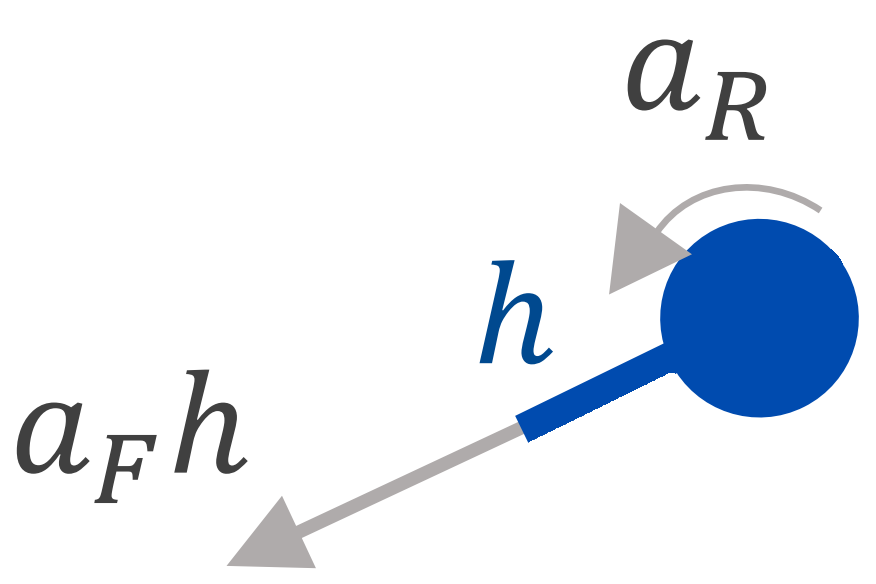
\includegraphics[width=\textwidth]{agent_active.png}
        %\caption{Active forces.}
        %\label{fig:image1}
    \end{minipage}
    \begin{minipage}{0.25\textwidth}
        \centering
        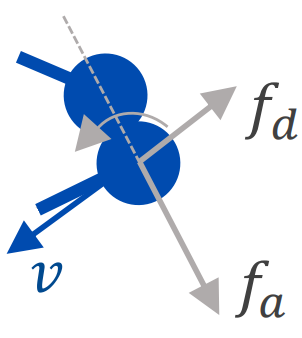
\includegraphics[width=\textwidth]{agent_passive.png}
        %\caption{Passive forces.}
        %\label{fig:image2}
    \end{minipage}
    \caption{Active (left) and passive (right) agent forces. \cite{li2023predator}}
    \label{fig:main_figure}
\end{figure}

At each time step, the simulation updates each agent's position and velocity by calculating the sum of the forces acting upon it. The overall dynamics governing these updates are given by:

$$ \dot{x} = v $$  
$$ \dot{v} = \frac{ha_F + F_d + F_a}{m} $$  
$$ \dot{\theta} = a_R $$  

Where:
\begin{itemize}
    \item $x \in \mathbb{R}^2$ is the agent's position,
    \item $v \in \mathbb{R}^2$ is the agent's velocity,
    \item $\theta \in [-\pi, \pi]$ is the agent's heading angle,
    \item $h \in \mathbb{R}^2$ is the unit vector representing the agent's heading direction, calculated as $h = [\cos(\theta), \sin(\theta)]^T$,
    \item $m \in \mathbb{R}$ is the agent's mass.\\
\end{itemize}

To better align the simulation with ant-like movement, rather than the smooth, bird-like flight patterns of the original framework, several parameters will require significant adjustments. Currently, settings like drag coefficient, stiffness coefficient, maximum forward acceleration, and rotational acceleration are optimized for smooth, continuous paths with limited turning ability and no halting, which emulates bird flight. To emulate the more abrupt, flexible movements characteristic of ants in a 2D bird's-eye view, we will modify these parameters. Specifically, we’ll increase rotational flexibility, reduce constraints on movement continuity, and adjust the ability to stop, giving agents more freedom in directional changes and pauses.

\subsection{Basic Reward Policy}

Our initial reward policy for producing social distancing patterns in agent behavior will focus solely on agent interaction. Social behavior will be encouraged by rewarding agents based on the number of nearby agents, which should lead to grouping behavior. Social distancing will be promoted by penalizing healthy agents for being near infected ones and vice versa. Specific reward and penalty values will be fine-tuned as we begin experimentation.

We plan to start with this simple reward policy before scaling up simulation complexity with more nuanced agent interactions. For example, we may introduce cooperative behavior by allowing agents to exchange resources or other benefits, which could model cooperative dynamics where agents work together to achieve common goals.

\subsection{Model Performance Measures}

To assess whether social distancing patterns emerge, we will transform agent interactions into a network and analyze the network structure, as demonstrated in \cite{Stroeymeyt2018}. We will focus on network statistics that impact disease transmission, including modularity (expected to decrease), clustering (expected to decrease), network efficiency (expected to increase), and degree centrality (expected to increase). Additionally, we will measure the average distance between agents, which will indicate whether agents are avoiding each other. These metrics will first be calculated in a network before the introduction of the pathogen to observe passive social distancing. After the pathogen is introduced, we will track how the network structure changes over time.

Emergent social distancing behavior should also be clearly observable in the simulation visualization. We expect healthy agents to avoid infected ones, and vice versa. This behavior will be especially evident if we increase the agent density within the environment. In such cases, we should observe infected agents becoming isolated, forming empty regions around them, while healthy agents fill the remaining space in the simulation.

\begin{figure}[hbt]
    \centering
    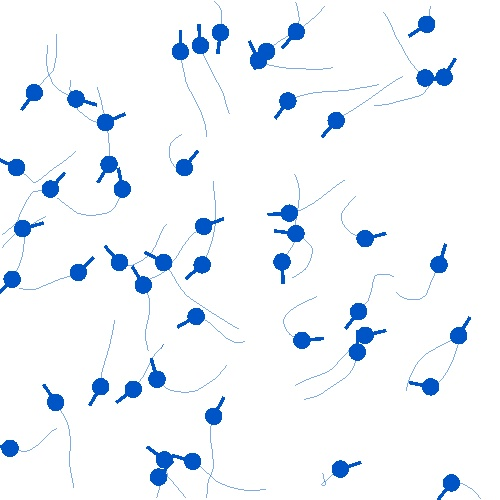
\includegraphics[width=0.75\linewidth]{figures/env_test_img.jpg}
    \caption{Simulation visualization example.}
    \label{fig:env_example}
\end{figure}

\section{Results}

As no experiments have been conducted yet, there are currently no results to present. Future updates will include analysis and findings based on the simulation outcomes, once experiments are underway.

\section{Discussion and Future Work}

As we have not yet obtained results, this section will outline our immediate plans and objectives leading up to the second report deadline.

Our primary goal is to adapt the existing reinforcement learning (RL) framework to align with our modeling objectives. This will involve the following steps:

\begin{enumerate}
    \item Agent Movement Adaptation: We will modify agent movement parameters to better simulate ant-like behavior. Current parameters are tuned for smoother, bird-like paths, whereas ants exhibit more abrupt, flexible movements. Adjustments will include increasing rotational flexibility, reducing constraints on movement continuity, and introducing options for sudden stops and directional changes.
    \item Policy Network Adjustment: We plan to reconfigure the policy network, which is the agent’s decision-making neural network. This network will be updated to process relevant environmental information and output appropriate actions for each agent based on its health status, position, and nearby agents. This customization will enable the agents to better respond to their surroundings, a necessary step for simulating disease-avoidance behaviors.
    \item Reward Policy Development: Our initial reward policy will be simple, rewarding agents for actions that minimize close interactions with infected agents and penalizing actions that lead to unnecessary contact. This will serve as a foundational incentive structure, helping us to examine how agents balance exploration with avoidance behaviors in a disease-prone environment.
\end{enumerate}

These steps will provide the basis for preliminary testing and fine-tuning. Moving forward, we plan to iterate on these adaptations and expand our focus to include more complex reward structures and interaction rules based on early observations from the simulations.

This organization clarifies each objective while positioning them as concrete steps. Additionally, the phrasing of each component emphasizes the purpose behind each modification, making the progression toward expected outcomes more cohesive and actionable.

\printbibliography

\end{document}
